\documentclass[a4paper]{article}

% Global layout
\usepackage{fancyhdr, graphicx, hyperref, indentfirst, lastpage, setspace}
\usepackage[margin=40mm]{geometry}

% Encoding
\usepackage[utf8]{vntex, inputenc}
\usepackage[english]{babel}
\usepackage{amsmath, amssymb, gensymb}

% Better table
\usepackage{array, booktabs, multicol, multirow, siunitx, tabularx}

% Code space
\usepackage[dvipsnames]{xcolor}
\usepackage{tikz}
\usepackage[framemethod=tikz]{mdframed}
\usepackage{minted, verbatim} % needs --shell-escape flag and Pygments

% Graphics
\usepackage{caption, float}

% Page setup
\allowdisplaybreaks{} % to have page breaks inside align* environment
\hypersetup{urlcolor=blue,linkcolor=black,citecolor=red,colorlinks=true}
\usemintedstyle{emacs}
\numberwithin{equation}{section}
\renewcommand{\arraystretch}{1.2} % space between table rows

% Global style setup
\makeatletter % change font size for not having underfull hbox
\renewcommand\Huge{\@setfontsize\Huge{22pt}{18}}
\makeatother

\AtBeginDocument{\renewcommand*\contentsname{Contents}}
\AtBeginDocument{\renewcommand*\refname{References}}
%\usepackage{fancyhdr}
\setlength{\headheight}{40pt}
\pagestyle{fancy}
\fancyhead{} % clear all header fields
\fancyhead[L]{
  \begin{tabular}{rl}
    \begin{picture}(25,15)(0,0)
      \put(0,-8){
\includegraphics[width=8mm, height=8mm]{./assets/hcmut.png}}
    \end{picture}
    \begin{tabular}{l}
      \textbf{\bf \ttfamily University of Technology, Ho Chi Minh City}\\
      \textbf{\bf \ttfamily Faculty of Computer Science and Engineering}
    \end{tabular}
  \end{tabular}
}
\fancyhead[R]{
	\begin{tabular}{l}
		\tiny \bf \
		\tiny \bf
	\end{tabular}  }
\fancyfoot{} % clear all footer fields
%\fancyfoot[L]{\scriptsize \ttfamily Assignment for Operating system - Academic year 2020 - 2021}
\fancyfoot[R]{\scriptsize \ttfamily Page {\thepage}/\pageref{LastPage}}
\renewcommand{\headrulewidth}{0.3pt}
\renewcommand{\footrulewidth}{0.3pt}

%%%
\setcounter{secnumdepth}{4}
\setcounter{tocdepth}{3}
\makeatletter
\newcounter{subsubsubsection}[subsubsection]
\renewcommand\thesubsubsubsection{\thesubsubsection.\@alph\c@subsubsubsection}
\newcommand\subsubsubsection{\@startsection{subsubsubsection}{4}{\z@}%
                                     {-3.25ex\@plus% -1ex \@minus% -.2ex}%
                                     {1.5ex \@plus% .2ex}%
                                     {\normalfont\normalsize\bfseries}}}}
\newcommand*\l@subsubsubsection{\@dottedtocline{3}{10.0em}{4.1em}}
\newcommand*{\subsubsubsectionmark}[1]{}
\makeatother

\setlength{\parindent}{1em}
\setlength{\parskip}{1em}
%\doublespacing
\begin{document}

\begin{titlepage}
  \begin{center}
    VIETNAM NATIONAL UNIVERSITY, HO CHI MINH CITY \
    UNIVERSITY OF TECHNOLOGY \
    FACULTY OF COMPUTER SCIENCE AND ENGINEERING
  \end{center}

  \vspace{1cm}

  \begin{figure}[H]
    \begin{center}
      
\includegraphics[width=4.5cm]{./assets/hcmut.png}
    \end{center}
  \end{figure}

  \vspace{1cm}

  \begin{center}
    \addtolength{\leftskip}{-0.3\textwidth}
    \addtolength{\rightskip}{-0.3\textwidth}
    \begin{tabular}{c}
      \textbf{\Large DATABASE SYSTEMS LAB (CO2014)} \\
      {}                                            \\
      \midrule                                      \\
      \textbf{\Large Assignment 2 Report}           \\
      {}                                            \\
      \textbf{\Huge HOSPITAL MANAGEMENT SYSTEM}     \\
      {}                                            \\
      \bottomrule
    \end{tabular}
  \end{center}

  \vspace{2cm}

  \begin{table}[h]
    \begin{tabular}{rll}
      \hspace{5cm} Advisor:  & Dr.\ Trần Minh Quang           \\
                             &                                \\
      \hspace{5cm} Class:    & CC08                           \\
      \hspace{5cm} Students: & Nguyễn Hoàng         & 1952255 \\
                             & Cao Bá Huy           & 1952713 \\
                             & Lưu Chấn Hưng        & 1952063
    \end{tabular}
  \end{table}

  \begin{center}
    {\footnotesize \large HO CHI MINH CITY, NOVEMBER 2021}
  \end{center}
\end{titlepage}

%\thispagestyle{empty}

\newpage
\tableofcontents
\newpage

\section{Improvement}
Recalling from our previous Hospital management database, we think that we can make some improvements to make our database more suitable to be used in real life hospitals. Therefore, we will make some changes by adding some constraints between some specific entities:

\begin{itemize}
  \item Firstly, a patient may be diagnosed with many diseases at the same time. Thus, we will let the attribute \textcolor{blue}{Diagnosis} in the \textcolor{blue}{PATIENT RECORD} be a multivalued attribute.
  \item Secondly, we will add a relationship called \textcolor{blue}{Provide} between \textcolor{blue}{DOCTOR} and \textcolor{blue}{TREATMENT}\@. A Doctor can provide many treatments.

  \item Thirdly, we add a relationship called \textcolor{blue}{Join} between \textcolor{blue}{DOCTOR} and \textcolor{blue}{APPOINTMENT}\@. A doctor may have one or many appointments, but an appointment is only joined by 1 doctor.
  \item Finally,  we add a relationship called \textcolor{blue}{Cost} between \textcolor{blue}{TREATMENT} and \textcolor{blue}{PAYMENT}\@. A treatment will only cost a payment.

\end{itemize}

That is all about our improvement, in the next section will discuss about the normal forms and modify the tables as well as the logical design.
\section{Normalization checking}
\subsection{Checking for violation of first normal form}
\subsubsection{Definition of first normal form }
\begin{itemize}
  \item \textcolor{blue}{First normal form (1NF)} is considered to be part of the formal definition of a relation in the basic (flat) relational model; historically, it was defined to disallow multivalued attributes, composite attributes, and their combinations.
  \item It states that the domain of an attribute must include only atomic (simple, indivisible) values and that the value of any attribute in a tuple must be a single value from the domain of that attribute.
  \item Hence, 1NF disallows having a set of values, a tuple of values, or a
        combination of both as an attribute value for a single tuple. In other words, 1NF
        disallows relations within relations or relations as attribute values within tuples. The
        only attribute values permitted by 1NF are single \textcolor{blue}{atomic (or indivisible) values}.
\end{itemize}

\subsubsection{Determine the violations}
In our design, we have a multivalued attribute called \textcolor{blue}{maintenance date}. This attribute belongs to the relation \textcolor{blue}{MEDICAL EQUIPMENT} and stores the date(s) this medical equipment got checked to assure it functions normally. \\
Moreover, we still have another multivalued attribute called \textcolor{blue}{Diagnosis} from the \textcolor{blue}{PATIENT RECORD} which we just added on the above section that violates 1NF\@.


\subsubsection{Solution}
First of all we will determine the violation of \textcolor{blue}{MEDICAL EQUIPMENT} relation because the attribute called \textcolor{blue}{Maintenance dates} stores a set of value, there by violating the 1NF\@.
\begin{figure}[H]
  \centering
  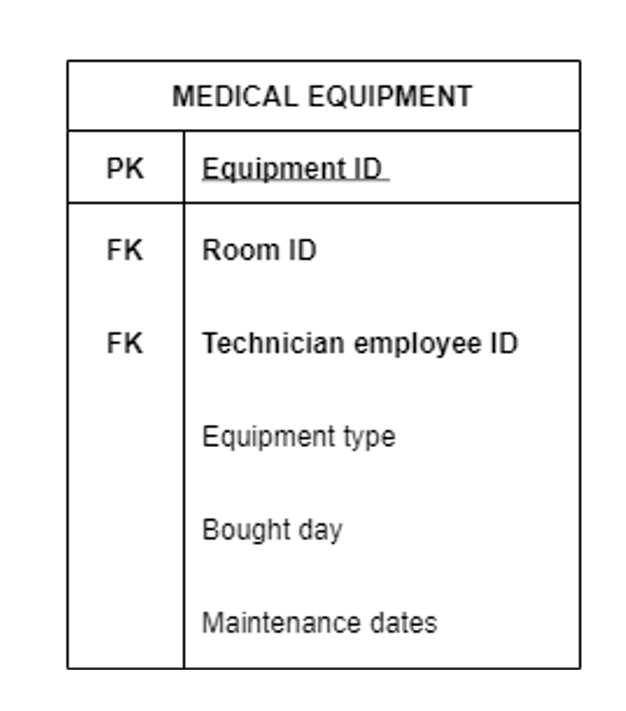
\includegraphics[width = 4cm ]{assets/1NFviolation.PNG}
  \caption{MEDICAL EQUIPMENT relation violates the 1NF }
\end{figure}

Next, we will remove the attribute \textcolor{blue}{Maintenance date} and create another relation called \textcolor{blue}{EQUIPMENT MAINTENANCE DATE} which includes the PK \textcolor{blue}{Equipment ID} from the \textcolor{blue}{MEDICAL EQUIPMENT} and the attribute called \textcolor{blue}{Date}. The primary key of this relation is the combination of 2 mentioned attributes: \textcolor{blue}{\{Date, Equipment ID\}}.

\begin{figure}[H]
  \centering
  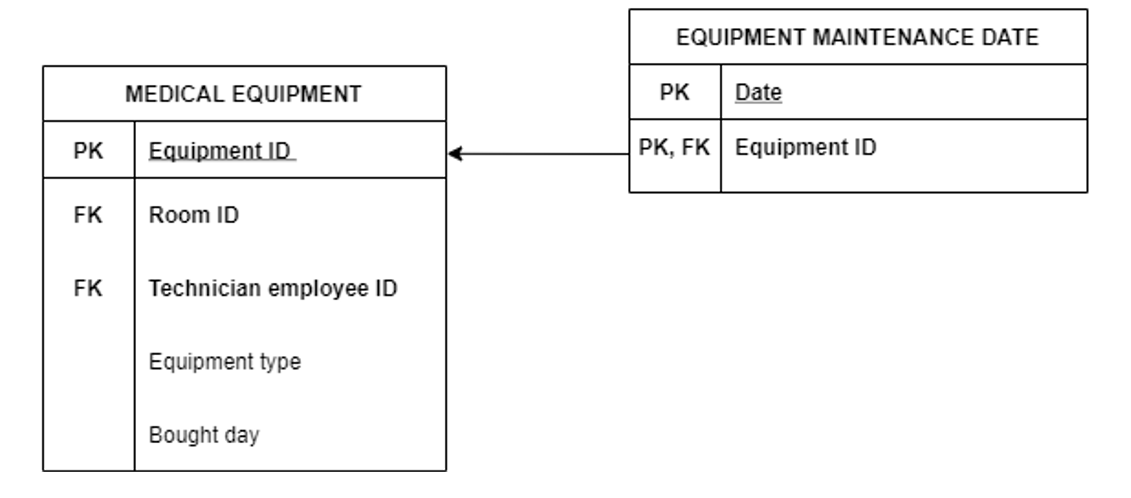
\includegraphics[width = 8cm ]{assets/1NFsolution.PNG}
  \captionsetup{justification=centering,margin=2cm}
  \caption{The result tables after we remove the attribute Maintenance date and create a new table to assure 1NF }
\end{figure}

Moreover, we still have another multivalued attribute called \textcolor{blue}{Diagnosis} from the \textcolor{blue}{PATIENT RECORD}\@.
Similarly, we will perform the same steps as above. We will first remove the attribute \textcolor{blue}{Diagnosis} and create another relation called \textcolor{blue}{PATIENT DIAGNOSIS} which includes the PK \textcolor{blue}{Record ID} from the \textcolor{blue}{PATIENT RECORD} table and the attribute called \textcolor{blue}{Diagnosis}. The primary key of this relation is the combination of 2 mentioned attributes: \textcolor{blue}{\{Diagnosis, Record ID\}}.
% figure 3
\begin{figure}[H]
  \centering
  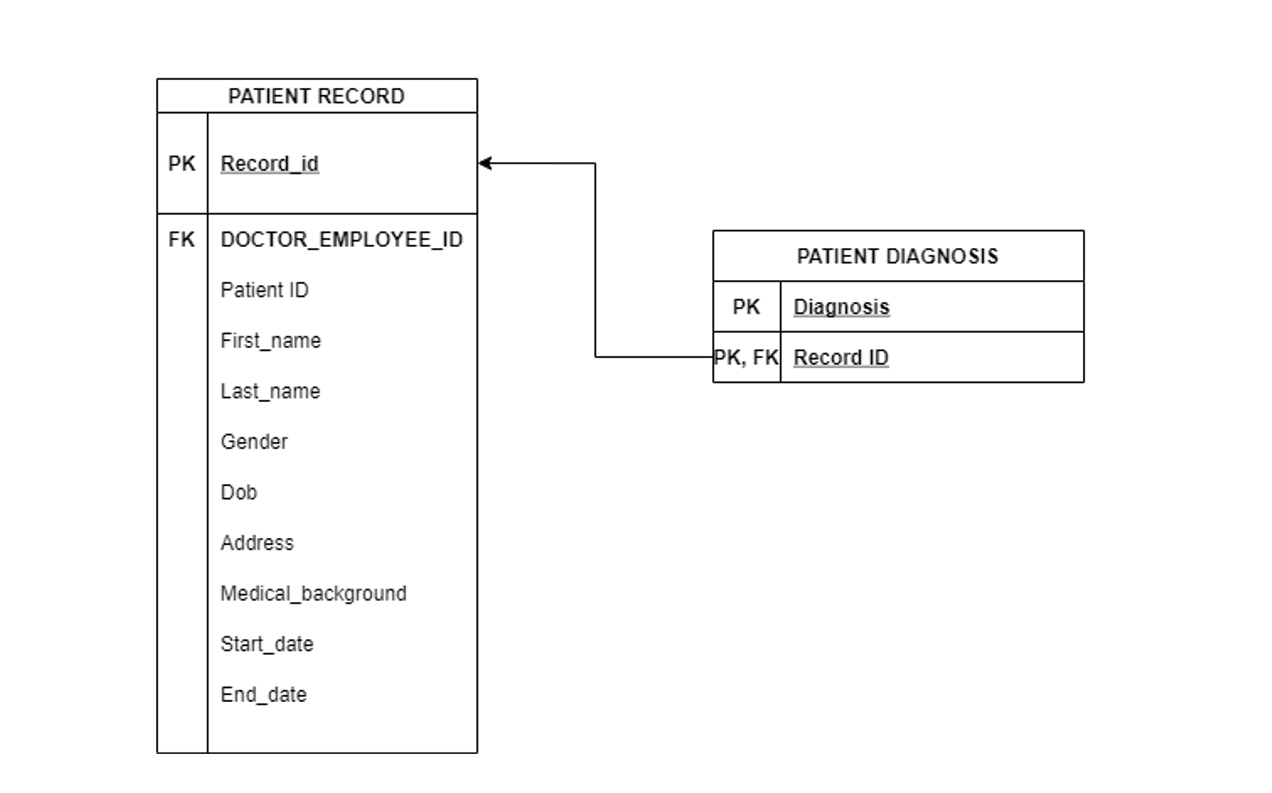
\includegraphics[width = 8cm ]{assets/1NFsolution2.PNG}
  \captionsetup{justification=centering,margin=2cm}
  \caption{The result tables after we remove the attribute \textcolor{blue}{Diagnosis} and create a new table to assure 1NF}
\end{figure}


\subsection{Checking for violation of second normal form}
\subsubsection{Definition of second normal form }
\textcolor{blue}{Second normal form (2NF)} is based on the concept of full functional dependency.
A functional dependency X \(\rightarrow \) Y is a full functional dependency if removal of any attribute A from X means that the dependency does not hold anymore; that is, for any attribute A \(\epsilon \) X, (X - \{A\}) does not functionally determine Y. \\
\(\Rightarrow \) A relation schema R is in 2NF if every non-prime attribute A in R is
fully functionally dependent on the primary key of R.

\subsubsection{Determine the violations}
Luckily, we can say that for each relation in our database, every non-prime attributes are fully dependent on the their respective primary key. Therefore, we can proudly say that our database is in 2NF\@.


\subsection{Checking for violation of third normal form}
\subsubsection{Definition of third normal form}
\textcolor{blue}{Third normal form (3NF)} is based on the concept of transitive dependency. A functional dependency X \(\rightarrow \) Y in a relation schema R is a transitive dependency if there exists a set of attributes Z in R that is neither a candidate key nor a subset of any key of  and both X \(\rightarrow \) Z and Z \(\rightarrow \) Y hold. \\
\(\Rightarrow \) According to Codd’s original definition, a relation schema R is in
\textcolor{blue}{3NF} if it satisfies 2NF and no non-prime attribute of R is transitively dependent on the primary key.

\subsubsection{Determine the violations}
In our design, the \textcolor{blue}{PATIENT RECORD} has violated the 3NF\@.
\begin{figure}[H]
  \centering
  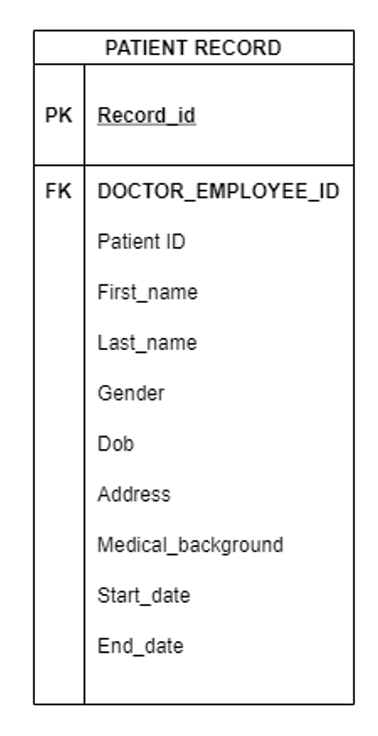
\includegraphics[width = 4cm ]{assets/3NFviolation.PNG}
  \caption{The \textcolor{blue}{PATIENT RECORD} relation}
\end{figure}

This relation is in 2NF but not in 3NF because of the transitive
dependency. To be more specific, we have the following dependencies:  \begin{itemize}
  \item Record ID \(\rightarrow \) \{patient ID, Doctor employee ID ,first name, last name,DOB, gender,address, medical background, start date, end date\}
  \item Patient ID \(\rightarrow \) \{first name, last name, dob, gender, address\}
\end{itemize}
This relation is not in 3F bcause of the transitive dependency of \textcolor{blue}{first name}, \textcolor{blue}{last name}, \textcolor{blue}{day of birth }, \textcolor{blue}{gender} and \textcolor{blue}{address} on \textcolor{blue}{Record ID} via \textcolor{blue}{Patient ID} (\textcolor{blue}{Patient ID} is a non-prime attribute).

\subsubsection{Solution}
We can normalize \textcolor{blue}{PATIENT RECORD} relations by decomposing it into the two 3NF relation schemas:
\begin{itemize}
  \item The first relation schema will be R1(Patient ID, Name,DOB, Gender, Address) where the \textcolor{blue}{Patient ID} is the primary key.
  \item The second relation schema will be R2(Record ID,Doctor employee ID, Patient ID, Medical background,start date, end date) where \textcolor{blue}{Record ID} is the primary key and \textcolor{blue}{Patient ID} is the foreign key that refers to primary key of R1.
\end{itemize}
\pagebreak
\begin{figure}[H]
  \centering
  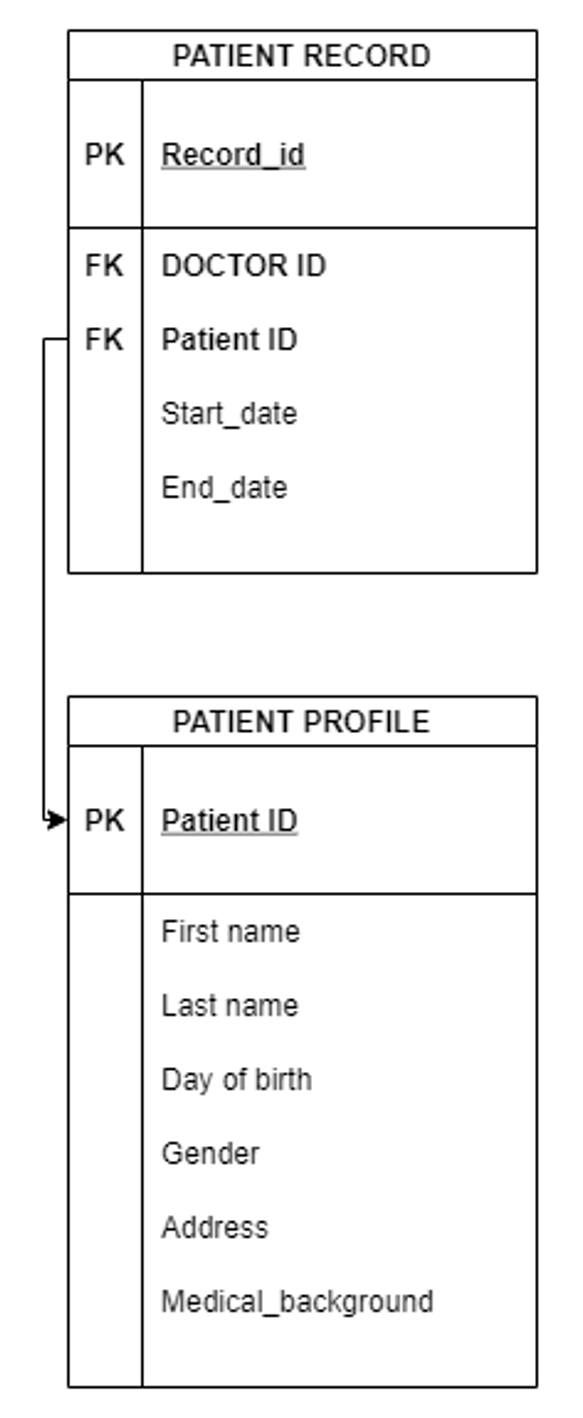
\includegraphics[width = 3cm ]{assets/3NFsolution.PNG}
  \captionsetup{justification=centering,margin=2cm}
  \caption{The decomposition of the \textcolor{blue}{MEDICAL RECORD} table into 2 tables.}
\end{figure}

\section{New logical design and physical}

\begin{figure}[H]
  \centering
  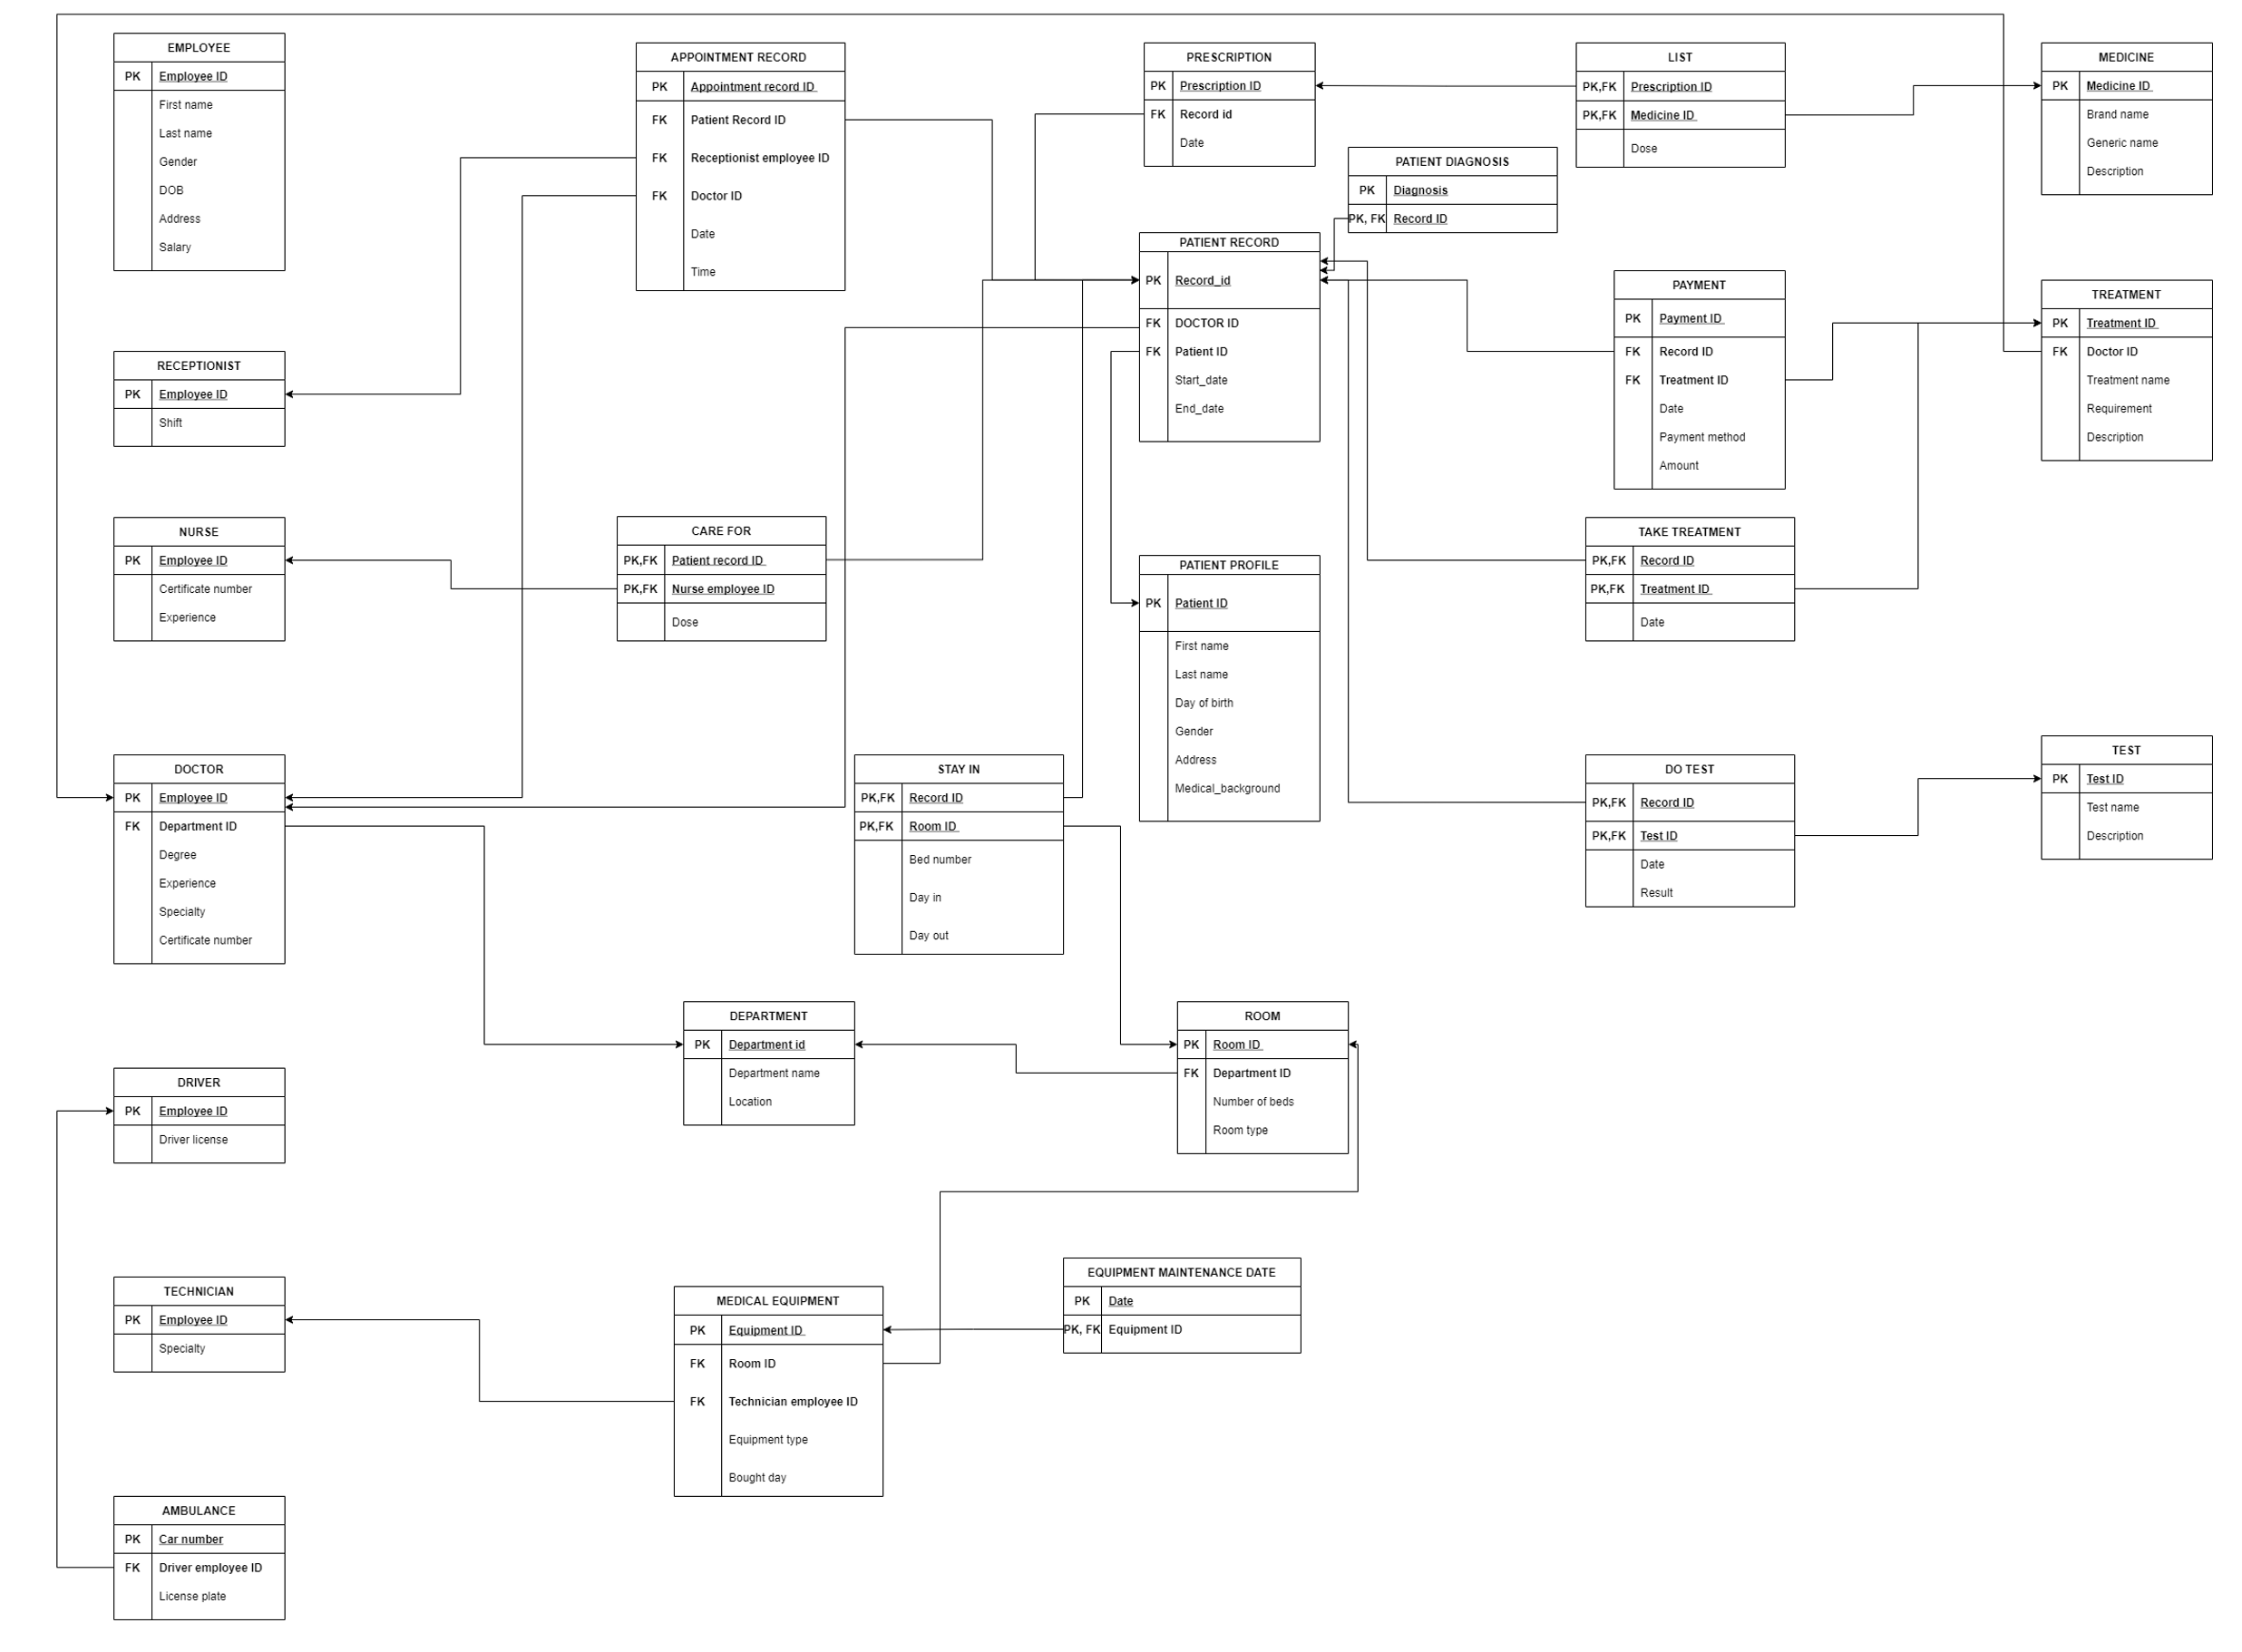
\includegraphics[width = 12cm ]{assets/newLogicalDesign.png}
  \captionsetup{justification=centering,margin=2cm}
  \caption{The new logical design that has been improved and assures all NFs}
\end{figure}

\newpage
\begin{figure}[H]
    \centering
    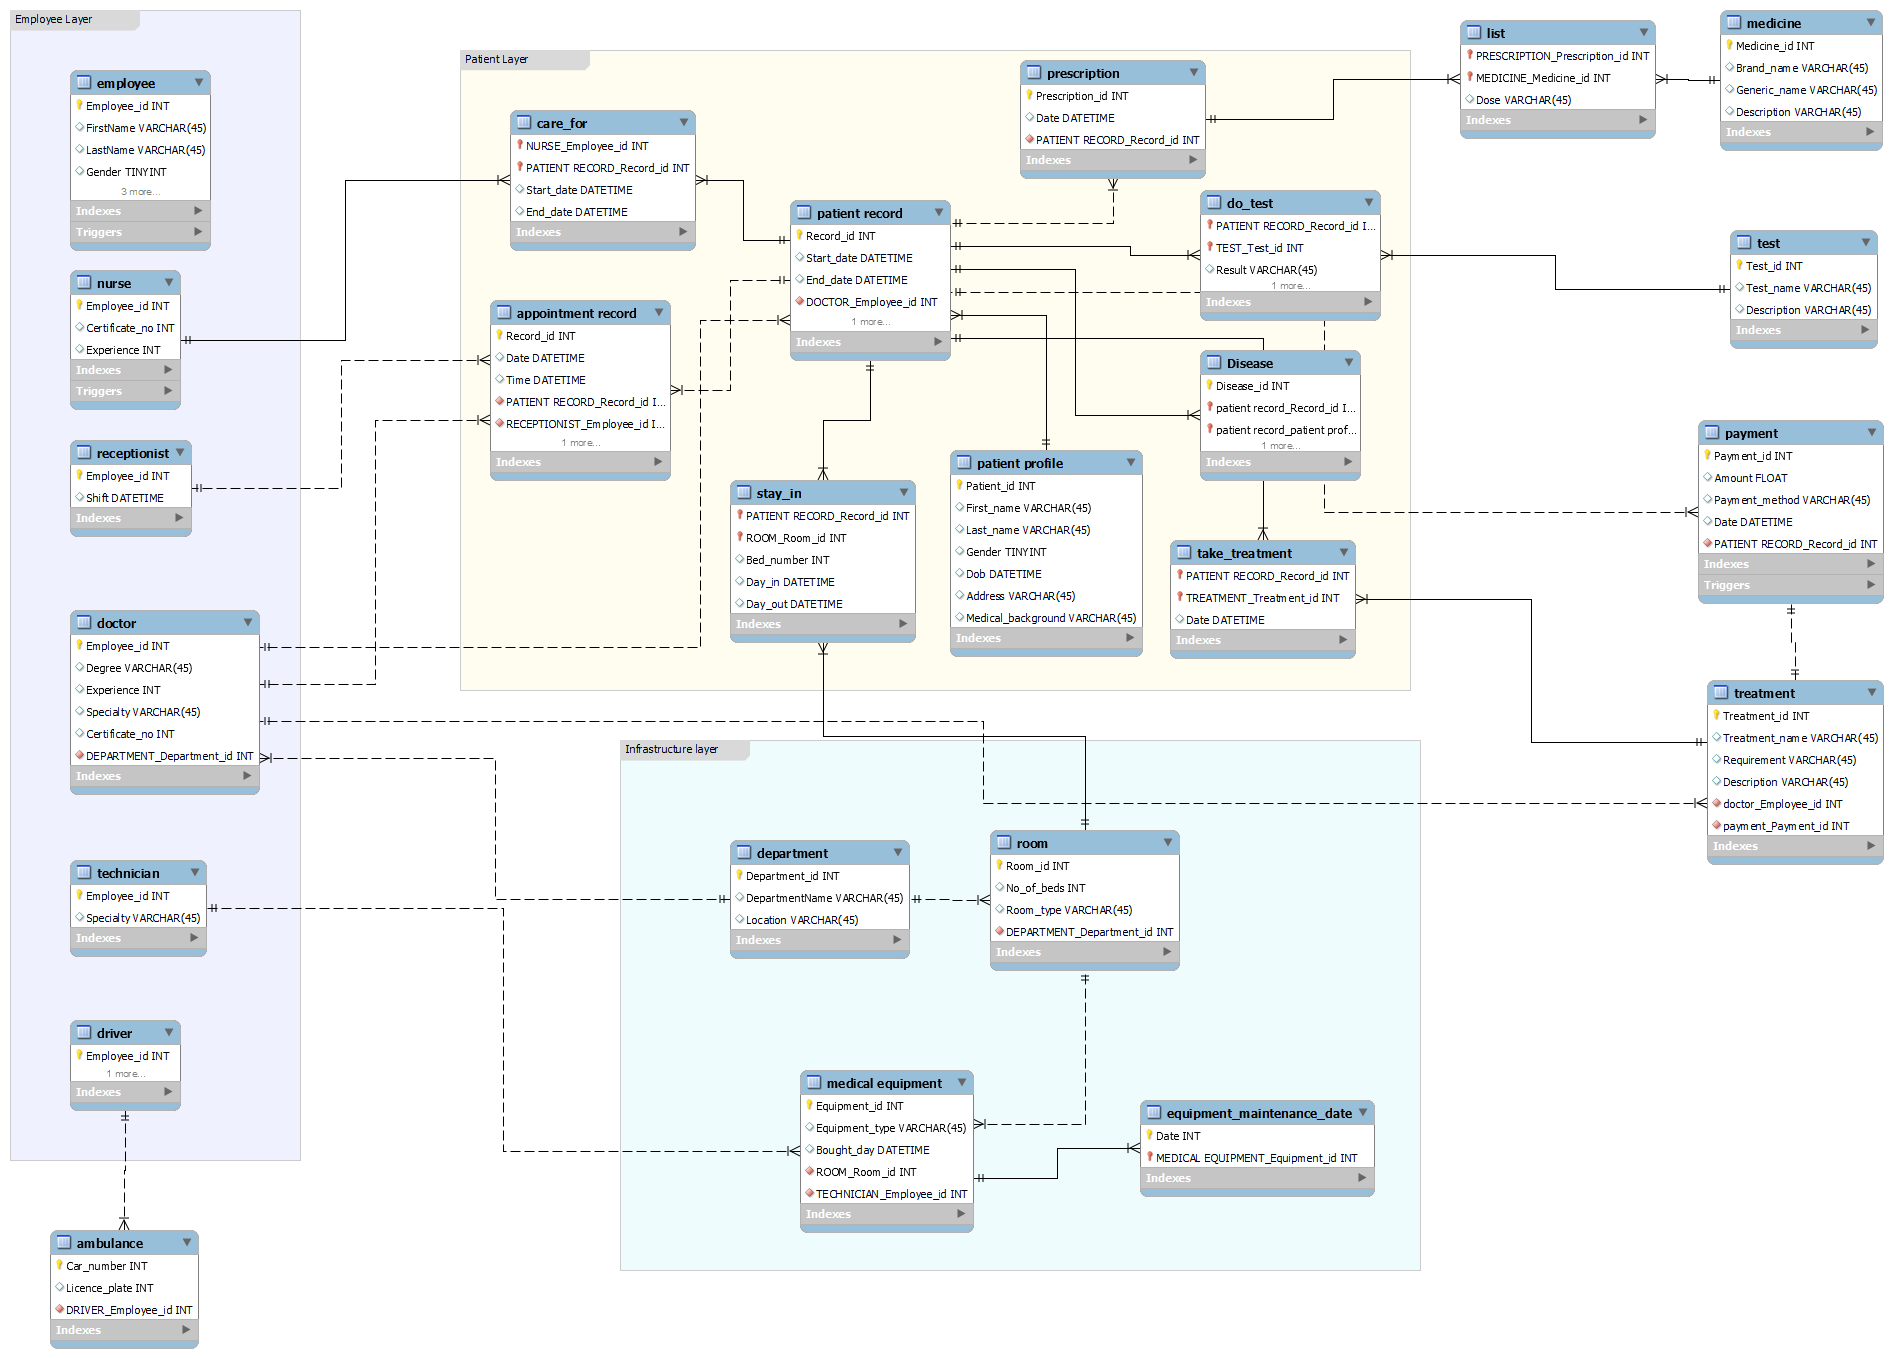
\includegraphics[width = 12cm]{assets/New_logcial_design.png}
    \captionsetup{justification=centering,margin=2cm}
    \caption{The new physical design implemented with MySQL Workbench}
\end{figure}

Similar to assignment 1, we will use a feature called \textcolor{blue}{Forward engineering } in MySQL workbench to convert the design to SQL code.  

\begin{figure}[H]
    \centering
    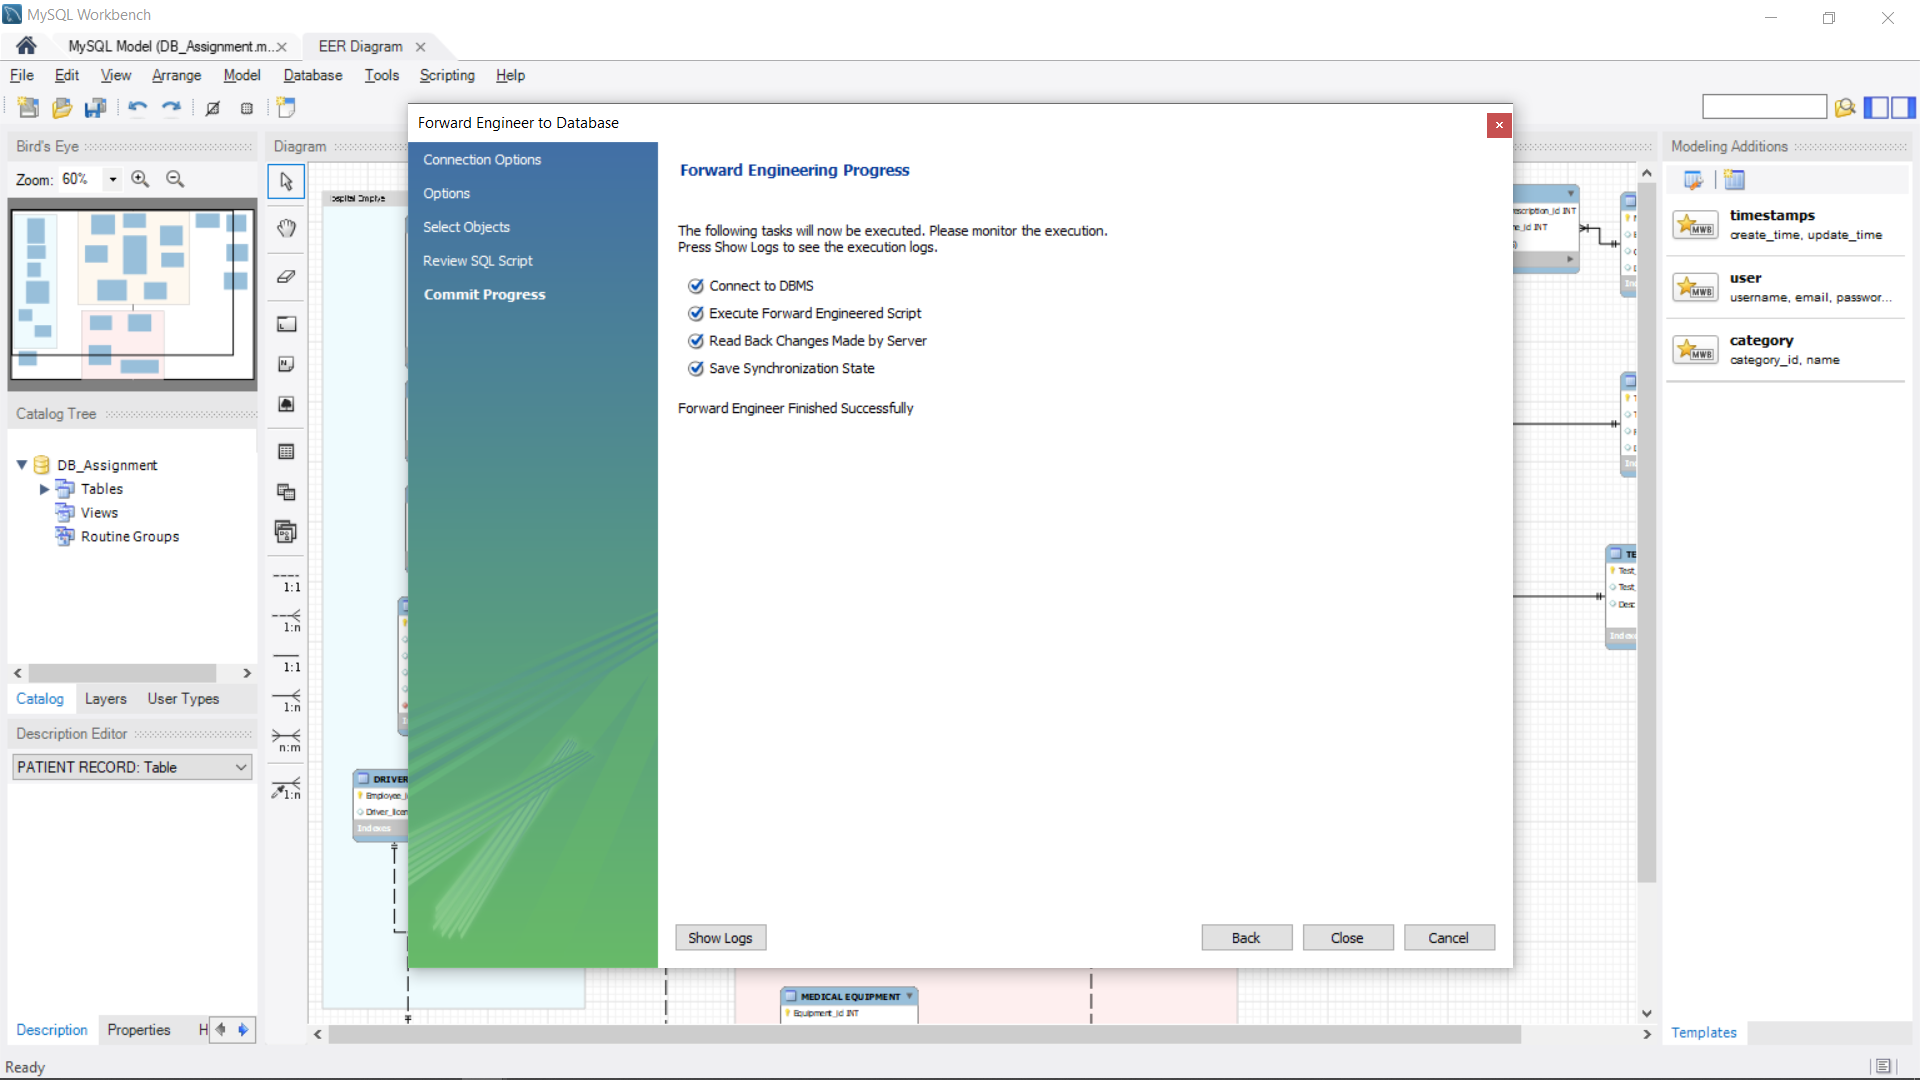
\includegraphics[width = 8cm]{assets/step2.png}
    \captionsetup{justification=centering,margin=2cm}
    \caption{Forward engineering finished successfully.}
\end{figure}
Our database is now ready to be used.


\pagebreak

\section{Implementation completion}

\subsection{Constraints specification}
First step to complete our implementation of the database is to complete a set of constraints, especially the referential integrity constraints of the foreign keys.
Luckily, MySQLWorkbench provides us with a simple interface to set these constraints.

\begin{figure}[H]
  \centering
  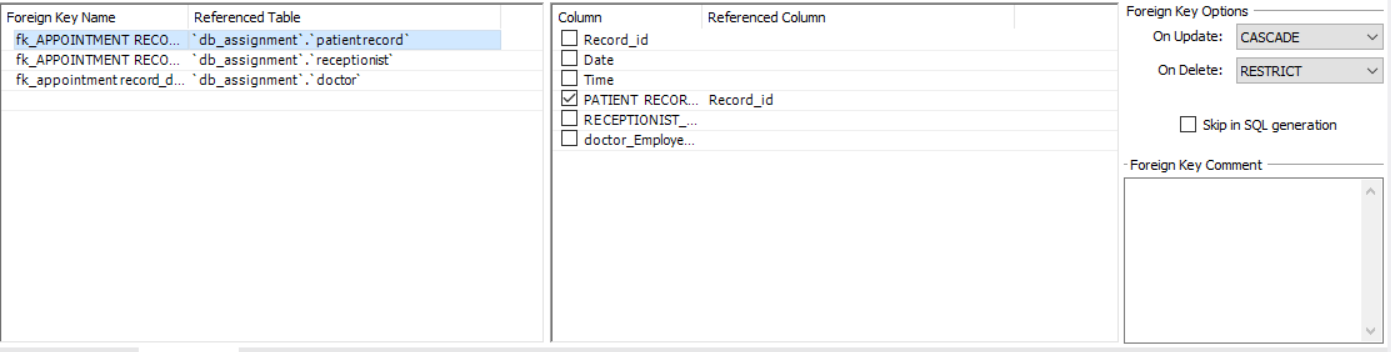
\includegraphics[width=0.8\textwidth]{assets/constraints_1.png}
  \captionsetup{justification=centering,margin=2cm}
  \caption{MySQL Workbench foreign keys options features}
\end{figure}

As we can see, the window on the right side allow us the ability to set the options when DELETE and UPDATE.We have 4 total options to choose (RESTRICT, CASCADE, SET NULL, NO ACTION).
Now we will have to go through each of our foreign keys and set the suitable option.

\begin{itemize}
  \item On \textcolor{blue}{DOCTOR} table, we have 1 FK referenced to \textcolor{blue}{DEPARTMENT} table.
        We would set CASCADE on both ON UPDATE AND ON DELETE.The reason for this choice is due to a business rule that when a \textcolor{blue}{DEPARTMENT} is removed, every doctors should be removed as well.
  \item For the rest of our tables, we would choose CASCADE ON UPDATE and RESTRICT ON DELETE\@.
        When the referenced table UPDATE their value, it is obvious that the referencing table should UPDATE as well, so we choose CASCADE ON UPDATE\@.
        For ON DELETE options, we choose RESTRICT because when a referenced table is deleted, we don't have to delete the referencing table as well because they represents two distinct entities.
\end{itemize}

\subsection{Triggers}

\subsubsection{Trigger on Employee's Salary}
The first trigger we would like to set is a constraint on the input of Salary column in EMPLOYEE table.
If a person wants to insert a negative value into our table, we would automatically set it to 0 as default.

\begin{figure}[H]
  \centering
  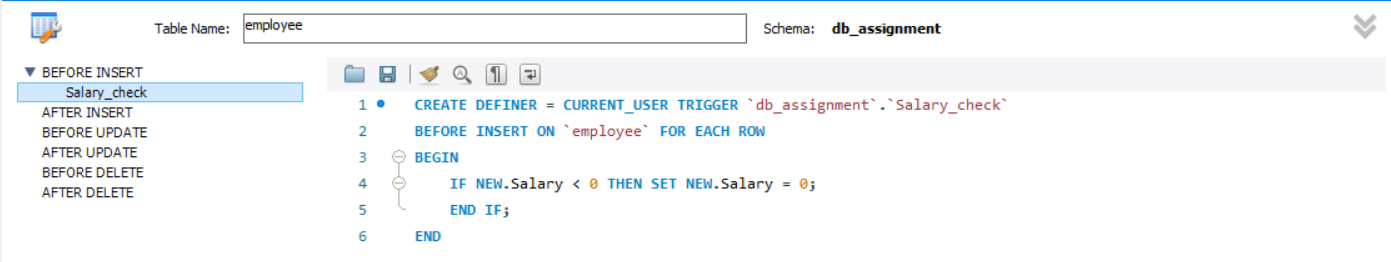
\includegraphics[width = 0.8\textwidth]{assets/trigger_1.png}
  \captionsetup{justification=centering,margin=2cm}
  \caption{Trigger on Employee's Salary}
\end{figure}

\subsubsection{Trigger on Experience of NURSE}
The second trigger is similar to the first one in terms of checking BEFORE\_INSERT constraint.
In this case, we would also set a default value of 0 whenever a person accidentally inserted a negative value of Experience column of NURSE table.

\begin{figure}[H]
  \centering
  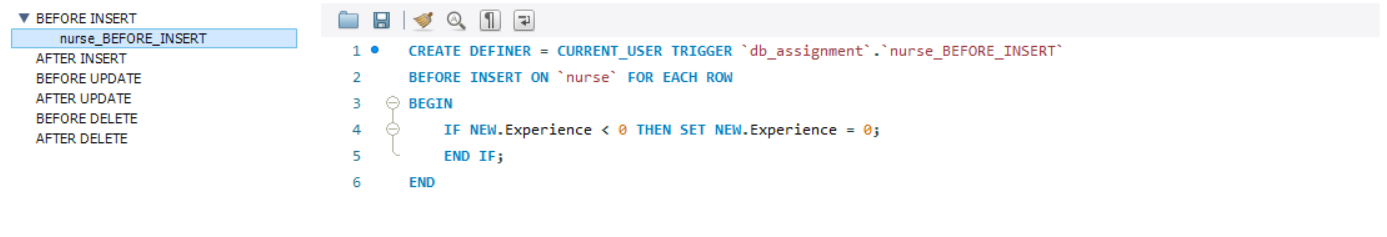
\includegraphics[width=0.8\textwidth]{assets/trigger_2.png}
  \captionsetup{justification=centering,margin=2cm}
  \caption{Trigger on Nurse's Experience}
\end{figure}

\subsubsection{Trigger on date of Appointment record}

The final trigger in our assignment is about the default value for a DATETIME type value, which is one of the most common usage of trigger.
We would create a trigger to automatically set the current date in to the

\begin{figure}[H]
  \centering
  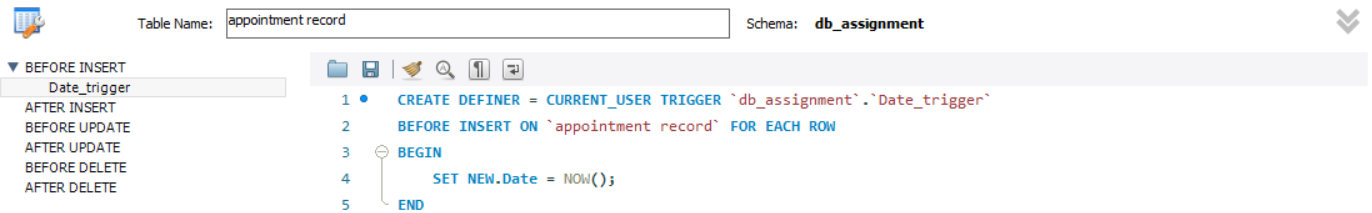
\includegraphics[width=0.8\textwidth]{assets/trigger_3.png}
  \captionsetup{justification=centering,margin=2cm}
  \caption{Trigger on Appointment Record}
\end{figure}

\subsection{Queries}

\subsubsection{Retrieve a full form of medical records}
As we mentioned earlier, one big improvement of our database after normalizing is the spilt of MEDICAL RECORD table into 2 sub tables, PATIENT PROFILE and PATIENT RECORD\@.
However, when we want to get the information of the whole medical record, we have to join those 2 table.

\begin{figure}[H]
  \centering
  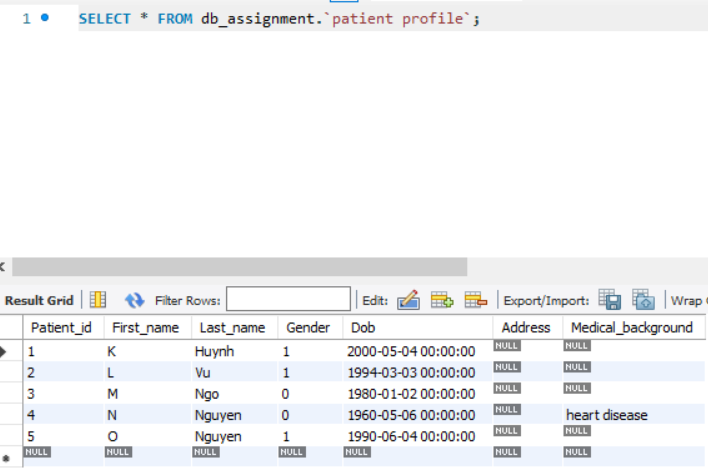
\includegraphics[width=0.8\textwidth]{assets/query_1c.png}
  \captionsetup{justification=centering,margin=2cm}
  \caption{PATIENT PROFILE table}
\end{figure}

\begin{figure}[H]
  \centering
  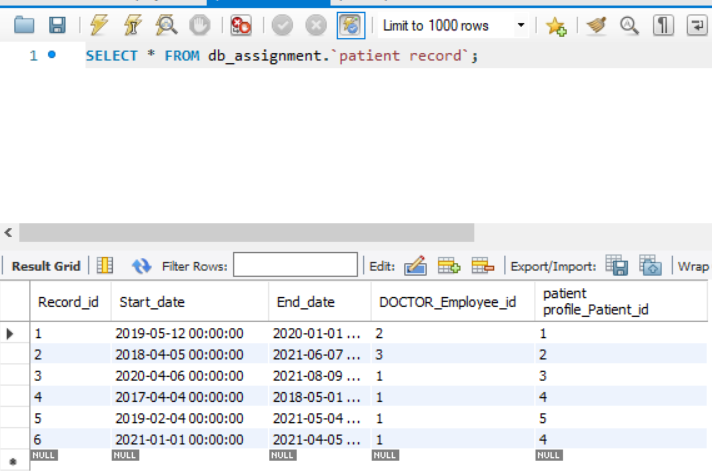
\includegraphics[width=0.8\textwidth]{assets/query_1b.png}
  \captionsetup{justification=centering,margin=2cm}
  \caption{PATIENT RECORD table}
\end{figure}

\begin{figure}[H]
  \centering
  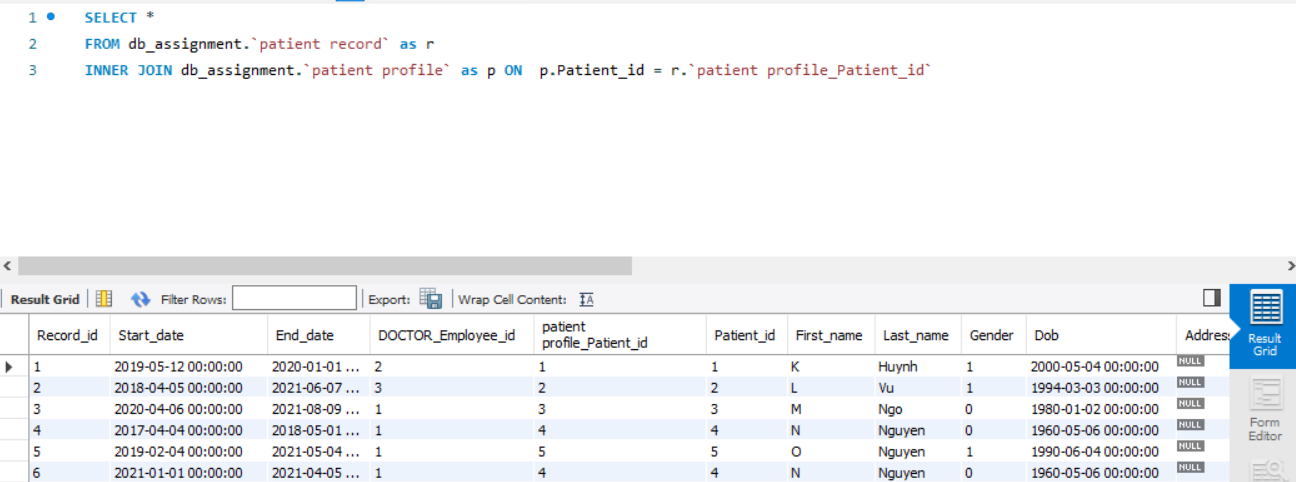
\includegraphics[width=0.8\textwidth]{assets/query_1a.png}
  \captionsetup{justification=centering,margin=2cm}
  \caption{Query and Result}
\end{figure}

As a result of the above query, we have a full form of a medical record.

\subsubsection{Get all prescriptions of patient ``Nguyen N'' }
In this query, we would like to retrieve all prescriptions of a patient named ``Nguyen N''.
As we already know, patient First name and Last name is stored in the PATIENT PROFILE table.While prescriptions are stored in PRESCRIPTION table, which have a foreign key referencing to Record id of PATIENT RECORD.Therefore, we first have to lookup the Record id of patient Nguyen N, then join with Prescription table on that Record id.

\begin{figure}[H]
  \centering
  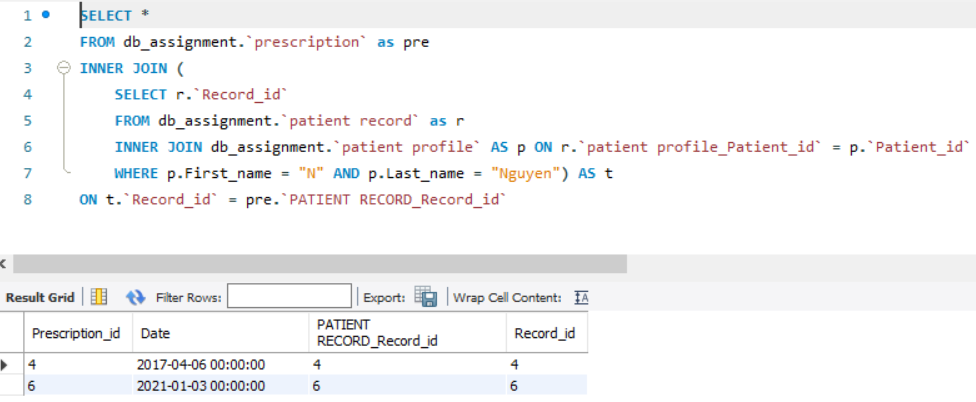
\includegraphics[width=0.8\textwidth]{assets/query_2.png}
  \captionsetup{justification=centering,margin=2cm}
  \caption{List of prescriptions used by Nguyen N}
\end{figure}

From the result we could conclude that Nguyen N has 2 prescriptions.

\subsubsection{Get the number patients treated by doctor ``Nguyen A''}

For the last query, we will get the number of patients treated by doctor Nguyen A.
From our database design, we know that employee names are stored in EMPLOYEE table.
Therefore, we have to find the Employee id of doctor Nguyen N, then find the number of patients treated by him.

\begin{figure}[H]
  \centering
  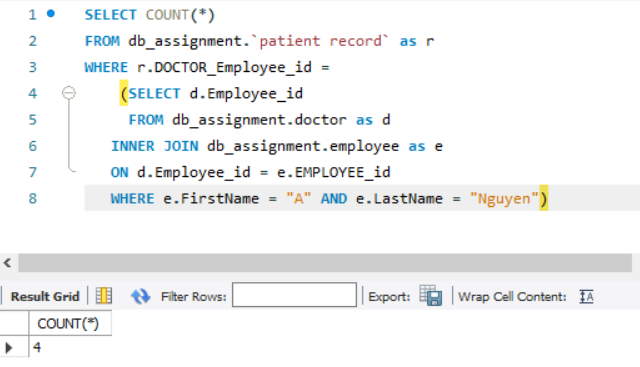
\includegraphics[width=0.8\textwidth]{assets/query_3a.png}
  \captionsetup{justification=centering,margin=2cm}
  \caption{Number of patients of doctor Nguyen A}
\end{figure}

\subsection{Stored procedures}

\subsubsection{Get monthly report of patient records}
For our first store procedure, we would like to store the query to retrieve the complete form of a medical record like the first query.
Because of that, we just need to store the query above into a procedures called Get\_report.

\begin{figure}[H]
  \centering
  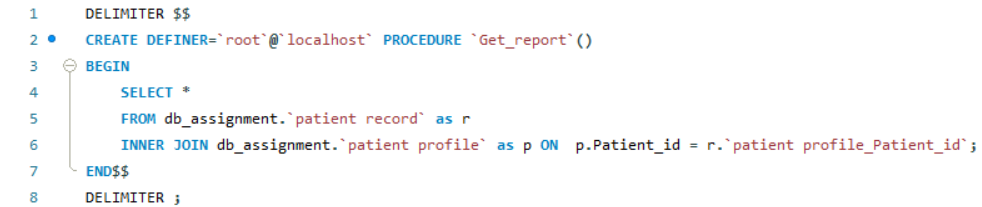
\includegraphics[width=0.8\textwidth]{assets/procedure_1a.png}
  \captionsetup{justification=centering,margin=2cm}
  \caption{Procedure creation code}
\end{figure}

\begin{figure}[H]
  \centering
  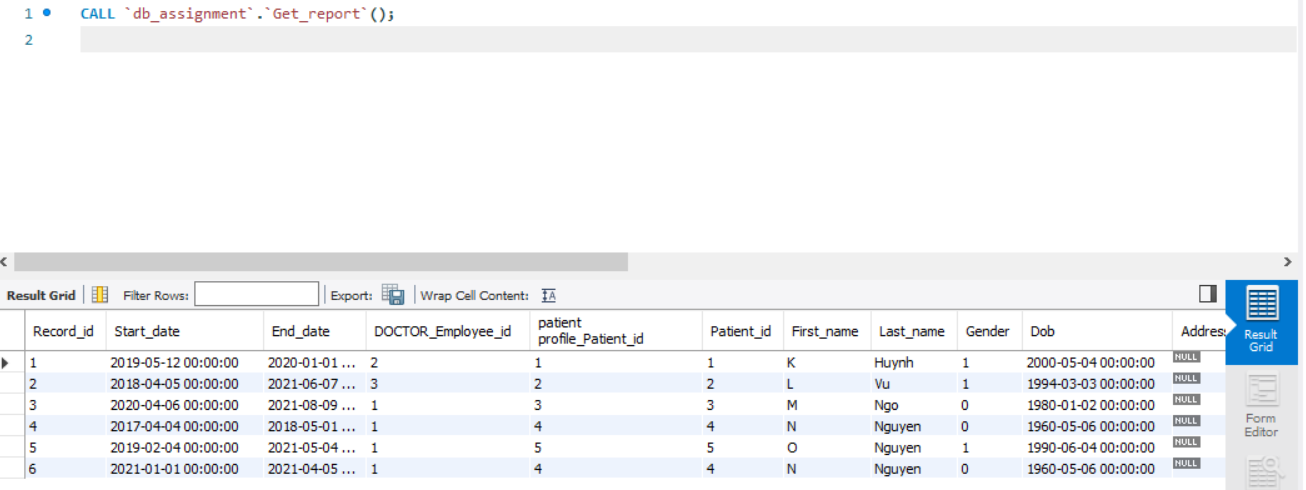
\includegraphics[width=0.8\textwidth]{assets/procedure_1b.png}
  \captionsetup{justification=centering,margin=2cm}
  \caption{Procedure call result}
\end{figure}

\subsubsection{Get number of patients stays in one department}

Next, a department would like to know how many patients have stayed in their building.
Therefore we create a procedure call named Get\_number\_of\_patients to get the number of patients stays in one department.Regarding the SQL code, we have to how many patients have stayed in which rooms that belongs to which department.

\begin{figure}[H]
  \centering
  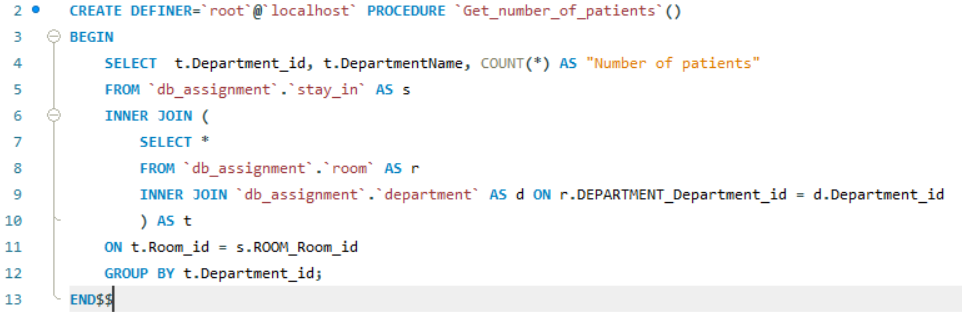
\includegraphics[width=0.8\textwidth]{assets/procedure_2a.png}
  \captionsetup{justification=centering,margin=2cm}
  \caption{Procedure creation}
\end{figure}

\begin{figure}[H]
  \centering
  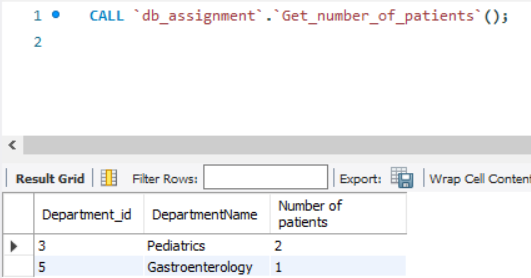
\includegraphics[width=0.8\textwidth]{assets/procedure_2b.png}
  \captionsetup{justification=centering,margin=2cm}
  \caption{Procedure call result}
\end{figure}
From the result, we could say that there are 2 patients stay in Pediatrics department and 1 patient stay in Gastroenterology department.

\subsubsection{Get a list of tests that were made by the hospital}
Last but no least, our final procedure is about getting a list of tests that were made by the hospital.
We know that a hospital conducts a lot of tests.
Therefore we have to get a report about all kinds of tests have been made.

\begin{figure}[H]
  \centering
  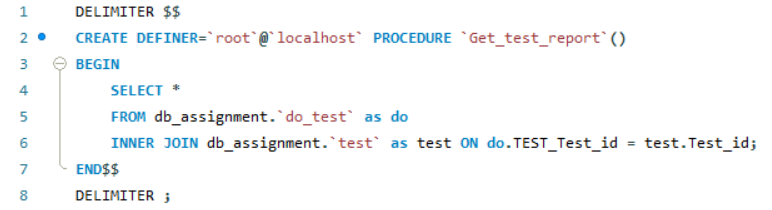
\includegraphics[width=0.8\textwidth]{assets/procedure_3a.png}
  \captionsetup{justification=centering,margin=2cm}
  \caption{Procedure call result}
\end{figure}

\begin{figure}[H]
  \centering
  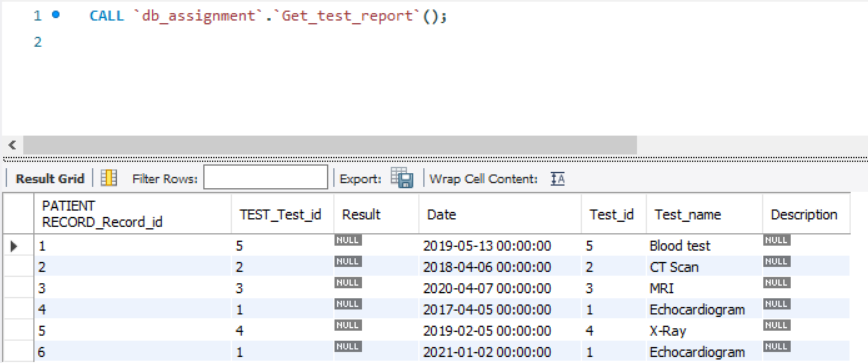
\includegraphics[width=0.8\textwidth]{assets/procedure_3b.png}
  \captionsetup{justification=centering,margin=2cm}
  \caption{Procedure call result}
\end{figure}

From our query, we could see the whole list of tests were conducted by the hospitals.


\section{Database security}
\subsection{Types of database security}
Database security is a broad area that addresses many issues, including the following:
\begin{itemize}
    \item  Various legal and ethical issues regarding the right to access certain information, for example, some information may be deemed to be private and cannot be accessed legally by unauthorized organizations or persons. 
    \item Policy issues at the governmental, institutional, or corporate level regarding what kinds of information should not be made publicly available, for example, credit ratings and personal medical records.
    \item System-related issues such as the system levels at which various security functions should be enforced, for example, whether a security function should be handled at the physical hardware level, the operating system level, or the DBMS level.
    \item The need in some organizations to identify multiple security levels and to categorize the data and users based on these classifications, for example, top secret, secret, confidential, and unclassified.
\end{itemize}

\subsection{Threats to databases}
Threats to databases can result in the loss of degradation of some or all of the following commonly accepted security goals:
\begin{itemize}
    \item  Loss of integrity: Database integrity refers to the requirement that information be protected from improper modification. Modification of data includes creating, inserting, and updating data; changing the status of data; and deleting data. Integrity is lost if unauthorized changes are made to the data by either intentional or accidental acts. If the loss of system or data integrity is not corrected, continued use of the contaminated system or corrupted data could result in inaccuracy, fraud, or erroneous decisions.
    \item Loss of availability. Database availability refers to making objects available to a human user or a program who/which has a legitimate right to those data objects. Loss of availability occurs when the user or program cannot access these objects.
    \item Loss of confidentiality. Database confidentiality refers to the protection of data from unauthorized disclosure. The impact of unauthorized disclosure of confidential information can range from violation of the Data Privacy Act to the jeopardization of national security. Unauthorized, unanticipated, or unintentional disclosure could result in loss of public confidence, embarrassment, or legal action against the organization.

\end{itemize}

\subsection{Solution}
When considering the threats facing databases, it is important to remember that the database management system alone cannot be responsible for maintaining the confidentiality, integrity, and availability of the data. Rather, the database works as a part of a network of services, including applications, Web servers, firewalls, SSL terminators, and security monitoring systems. Because security of an overall system is only as strong as its weakest link, a database may be compromised even if it would have been perfectly secure on its own merits. \\ \\
To protect databases against these types of threats, four kinds of countermeasures can be implemented: 
\begin{enumerate}
    \item Access control
    \item Inference control
    \item Flow control
    \item Data encryption
\end{enumerate}

\subsubsection{Access control}
A DBMS typically includes a database security and authorization subsystem that is responsible for ensuring the security of portions of a database against unauthorized access. It is now customary to refer to two types of database security mechanisms : 
\begin{itemize}
    \item \textcolor{blue}{Discretionary Access control}. These are used to grant privileges to users, including the capability to access specific data files, records, or fields in a specified mode (such as read, insert, delete, or update).
    \item \textcolor{blue}{Mandatory access control}. These are used to enforce multilevel security by classifying the data and users into various security classes (or levels) and then implementing the appropriate security policy of the organization. For example, a typical security policy is to permit users at a certain classification (or clearance) level to see only the data items classified at the user’s own (or lower) classification level. An extension of this is role-based security, which enforces policies and privileges based on the concept of organizational roles.
\end{itemize}

\subsubsection{Inference control}
Inference control in databases, also known as \textcolor{blue}{Statistical Disclosure Control (SDC)}, is a discipline that seeks to protect data so they can be published without revealing confidential information that can be linked to specific individuals among those to which the data correspond. SDC is applied to protect respondent privacy in areas such as official statistics, health statistics, e-commerce (sharing of consumer data), etc. Since data protection ultimately means data modification, the challenge for SDC is to achieve protection with minimum loss of the accuracy sought by database users.

\subsubsection{Data encryption}
A control measure is data encryption, which is used to protect sensitive data (such as credit card numbers) that is transmitted via some type of communications network. Encryption can be used to provide additional protection for sensitive portions of a database as well. The data is encoded using some coding algorithm. An unauthorized user who accesses encoded data will have difficulty deciphering it, but authorized users are given decoding or decrypting algorithms (or keys) to decipher the data.



\subsubsection{Flow control}
The flow control helps prevents information from flowing in such a way that it reaches unauthorized users.  A flow policy lists out the channels through which information can flow. It also defines security classes for data as well as transactions.

\newpage

\section{Develop an application on top of the Database system}
Any database system would expose an interface so that the users can hook on to this connection and perform tasks on the database.
The big problem is different databases require different properties for a connection to be established.
To not put a burden on the database users, we as developers need to do the technical work and only expose what the users need.

With that having been said, we decided to create a webserver that provides a RESTful API.
We will demonstrate the application on the \textcolor{blue}{AMBULANCE} table.
Our server lives at \url{localhost:3000} as seen here.
\begin{figure}[H]
    \centering
    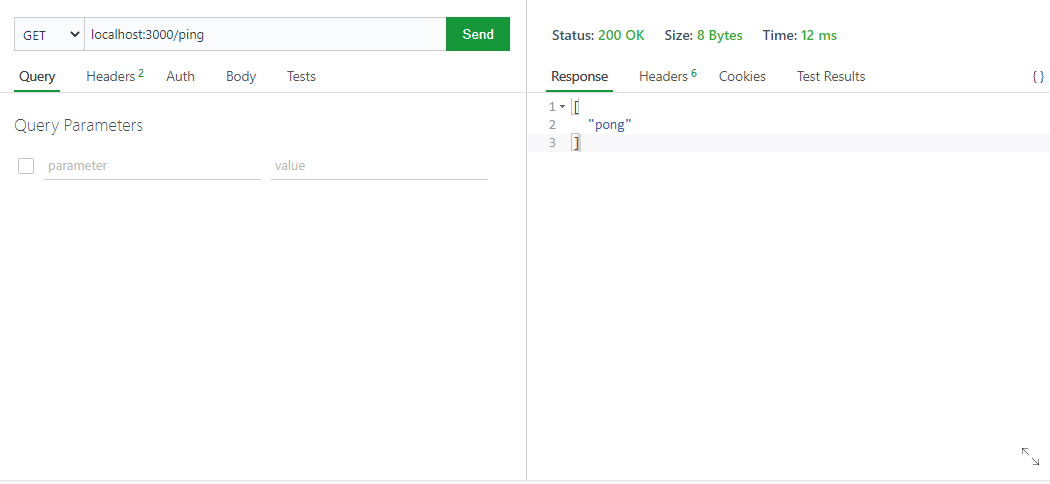
\includegraphics[width=0.8\textwidth]{./assets/api_ping.png}
    \caption{Test ping to the application}
\end{figure}

\begin{itemize}
    \item \textcolor{blue}{Create}:
    We will add data to the table at \textcolor{blue}{/ambulance/new} using POST method and form-data.
    We will insert 2 entries into the table.
    \begin{figure}[H]
        \centering
        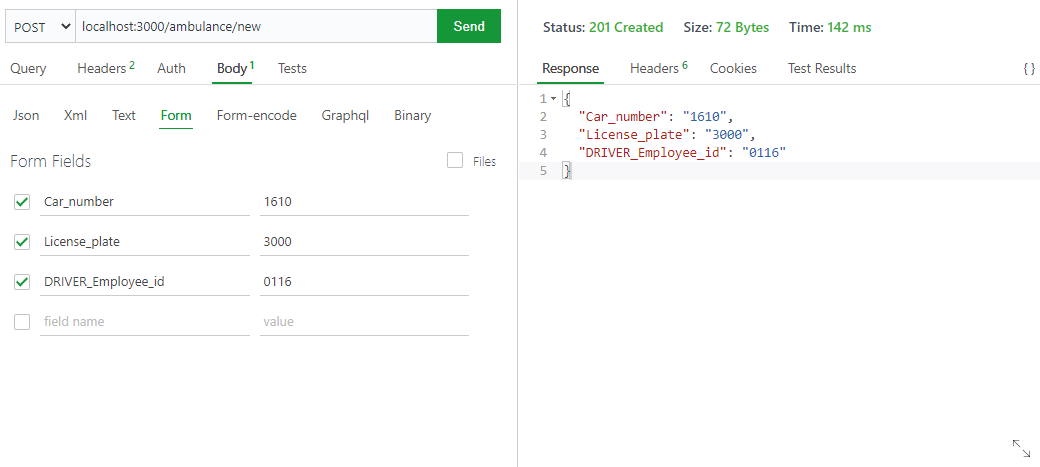
\includegraphics[width=0.8\textwidth]{./assets/api_new1.png}
        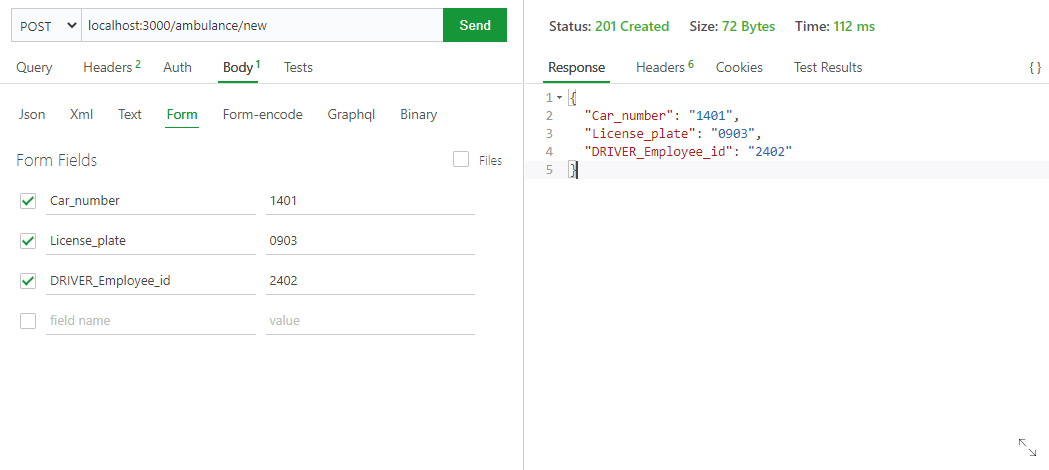
\includegraphics[width=0.8\textwidth]{./assets/api_new2.png}
        \caption{Adding entries to the table}
    \end{figure}
    
        \item \textcolor{blue}{Retrieve}:
    We will get data from the table at \textcolor{blue}{/ambulance/all} using GET method.
    \begin{figure}[H]
        \centering
        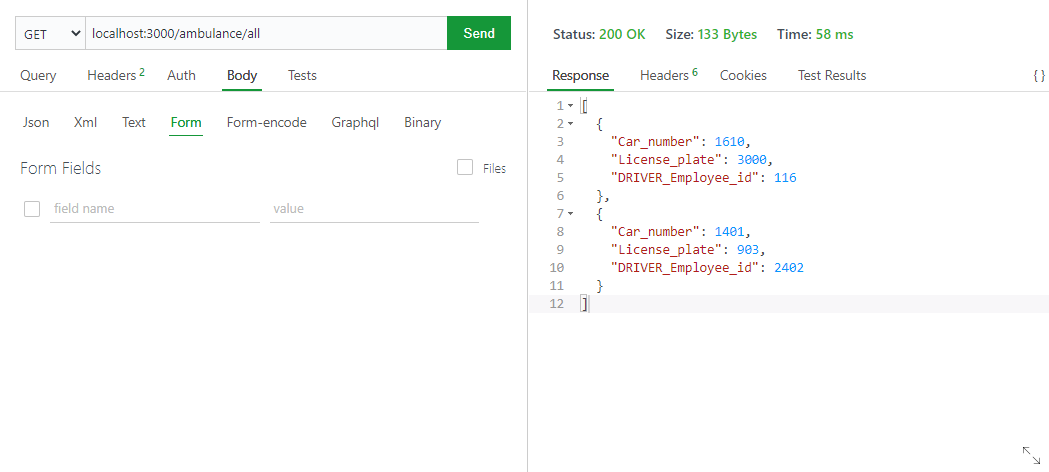
\includegraphics[width=0.8\textwidth]{./assets/api_all.png}
        \caption{Get all entries of table}
    \end{figure}
    
    We also provide a method to get data of one entry from the table at \textcolor{blue}{/ambulance/<Car\_number>} using GET method.
    \begin{figure}[H]
        \centering
        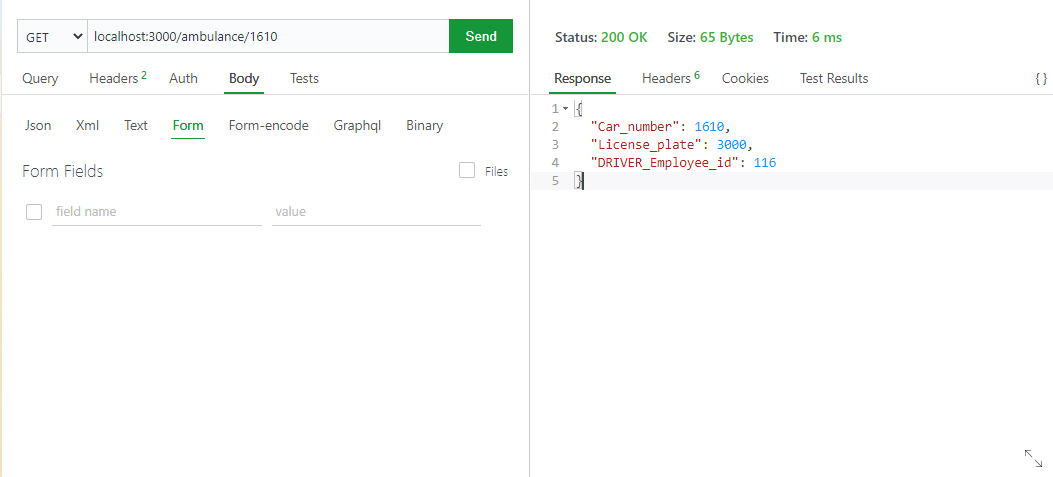
\includegraphics[width=0.8\textwidth]{./assets/api_one.png}
        \caption{Get one entry of table}
    \end{figure}
    
        \item \textcolor{blue}{Delete}:
    We will now remove one entry from the table at \textcolor{blue}{/ambulance/<Car\_number>/delete} using DELETE method.
    \begin{figure}[H]
        \centering
        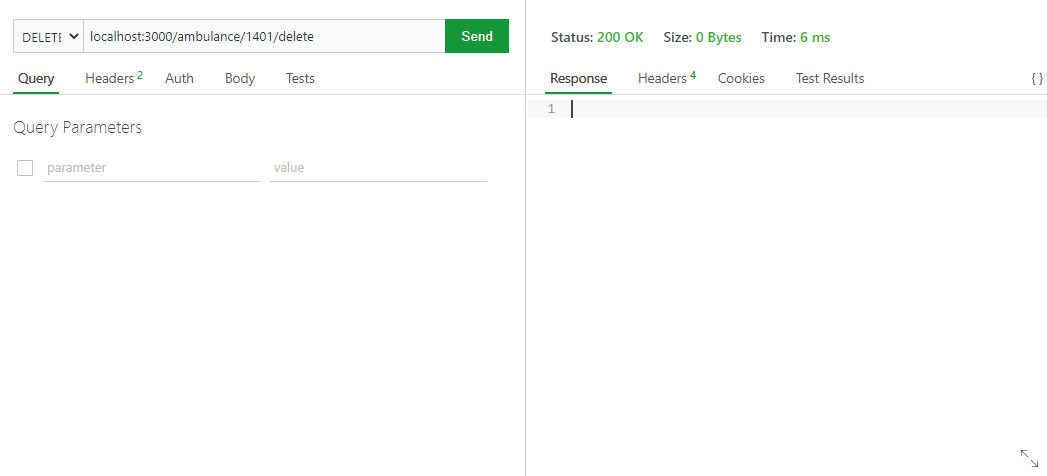
\includegraphics[width=0.8\textwidth]{./assets/api_delete.png}
        \caption{Delete the entry whose Car number is 1401 }
    \end{figure}
    
    We call \textcolor{blue}{/ambulance/all} again to verify that the entry has been deleted.
    \begin{figure}[H]
        \centering
        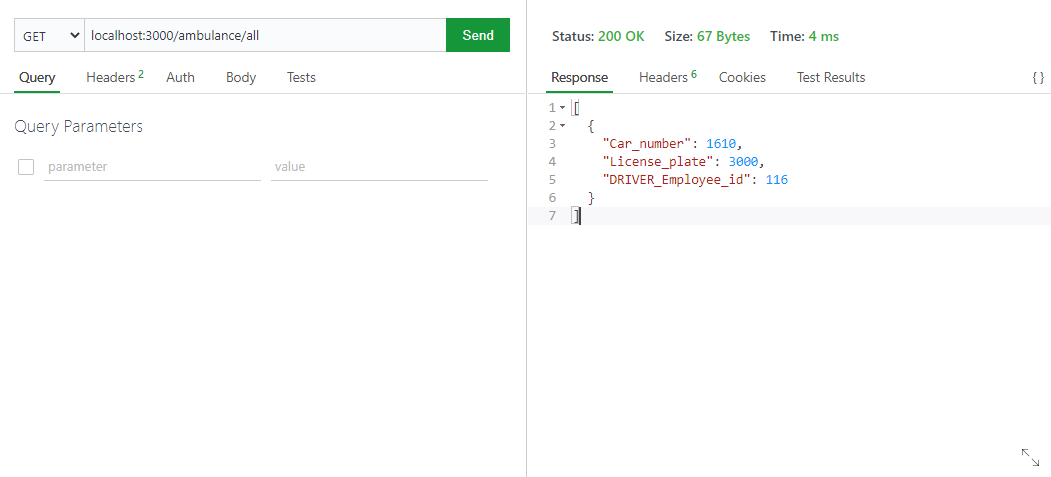
\includegraphics[width=0.8\textwidth]{./assets/api_all2.png}
        \caption{The result after we delete the entry whose Car number is 1401}
    \end{figure}
\end{itemize}

You can find the full source code at :  \url{https://github.com/Smithienious/CO2014-Asg/tree/dev/rest-api}

\section{Conclusion}
Through this assignment, we have learned how to improve our database and make it more suitable for business and real life uses. First of all, we have discussed about database normalization  and applied it straight away to our Hospital database management to reduce the redundant data and enhance the consistency of the whole database. Second of all, we have talked about the database security such as the types of database security, the security threats and some solutions that are usually considered to the database security problem. Finally, we have written some complex queries, triggers , stored procedures as well as create a simple application above this database. Therefore, we can say that although there are still many things to learn, accomplishing this assignment has surely helped us to understand clearer about the structure of a database as well as the process of designing databases in a logical way for business purposes.
       
\pagebreak
\begin{thebibliography}{9}
  \bibitem{texbook}
  R. Elmasri \& S.B. Navathe (2016): Fundamentals of Database Systems, 7th
  Edition, Addison-Wesley.
  
  \bibitem{textbook} 
  Nate Lord (2020) : Definiton of Data encryption, accessed with: \url{https://digitalguardian.com/blog/what-data-encryption}
  
  \bibitem{textbook}
  TutorialsPoint : Database security, accessed with : \url{https://www.tutorialspoint.com/distributed_dbms/distributed_dbms_database_security_cryptography.htm} 
  
  \bibitem{textbook}
  Josep Domingo-Ferrer, Inference Control in Statistical Databases, accessed with : \url{https://link.springer.com/referenceworkentry/10.1007\%2F978-0-387-39940-9_203}
  
  \bibitem{textbook}
  GeeksforGeeks: Different types of MySQL Triggers (with examples), accessed with: \url{https://www.geeksforgeeks.org/different-types-of-mysql-triggers-with-examples/}
  
  \bibitem{textbook}
  MySQL: Trigger Syntax and Examples, accessed with: \url{https://dev.mysql.com/doc/refman/8.0/en/trigger-syntax.html}
  
  \bibitem{textbook}
  W3school: SQL Stored Procedures for SQL Server, accessed with: \url{https://www.w3schools.com/sql/sql_stored_procedures.asp}
  
  % \bibitem{textbook}
  % Leslie Lamport (1994) \emph{\LaTeX: a document preparation system}, Addison
  % Wesley, Massachusetts, 2nd ed.
\end{thebibliography}




\end{document}
